\chapter{\MakeUppercase{Literature Review}}
\setcounter{equation}{0}

\section{\MakeUppercase{Current Approaches}}

\subsection{\MakeUppercase{Deblur-NeRF}}
Deblur-NeRF stands as a foundational method that extends the principles of 2D image deblurring into the 3D domain of NeRF. Its core innovation is the Deformable Sparse Kernel (DSK) module. This module jointly optimizes the NeRF scene representation and a dynamic blur kernel. By predicting a different kernel for different image regions, the DSK can adapt to complex, non-uniform blurs caused by camera motion or defocus, making it a powerful baseline for handling blurry multi-view images.\cite{bib3}

\subsection{\MakeUppercase{DP-NeRF}}
DP-NeRF approaches the deblurring problem by integrating physical scene priors into the model. It combines a rigid, physics-based blurring kernel with an adaptive weight protocol. This method leverages assumptions about the physical causes of blur to constrain the optimization process, aiming to enhance the quality and physical plausibility of the deblurred images used for NeRF training.

\subsection{\MakeUppercase{ActiveNeRF}}
ActiveNeRF introduces the concept of active learning to the NeRF ecosystem, but its primary focus differs from that of NeRF-DA. ActiveNeRF's data selection strategy is based on uncertainty estimation, which it achieves by computing the variance in the posterior distribution. This allows the model to request views from positions where its uncertainty about the scene is highest, making it effective for efficient scene exploration but not specifically tailored to the problem of blur.

\section{\MakeUppercase{Limitations of Existing Approaches}}

A major failing of existing deblurring methods like Deblur-NeRF is the lack of strategic management regarding the quantity and quality of blurred training samples. While Deblur-NeRF significantly advances the recovery of sharp Neural Radiance Fields (NeRFs) from blurry inputs, the conventional approach overlooked the impact of the degree of blurriness in the input data on the performance of the model. Training on the entire dataset often proves detrimental, as the overall results of Deblur-NeRF are significantly affected by the quantity of blurry training samples. Experiments have demonstrated that as the number of blurry images increases beyond a certain threshold, their utility in enhancing the model's performance decreases. In fact, utilizing the entire blurred image pool can actually slightly reduce performance. This redundancy and the inclusion of overly blurred or "useless views" necessitate active data curation, as incorporating all views, including highly blurred images, can actively hinder model performance. This highlights the need for an approach that focuses on selecting only high-quality blurred images for 3D scene modeling.

In addition to issues related to data quality and quantity, existing approaches do not adequately address the data imbalance inherent in light-field imagery. In practical applications capturing light field images with multi-view cameras, the prevalent central positioning of cameras causes considerable overlap in their fields of view, which can introduce blurring errors and adversely affect model performance. Furthermore, an imbalance exists between the center and the edges of the light field. Images captured with camera positions distant from the center of the light field may experience occlusions at their outer edges during the restoration process. Consequently, this information imbalance affects the learning process for the optimized ray of the edge pixel, resulting in relatively insufficient learning and occlusion in restoration compared to the learning of center pixels. Because capturing multi-view images in real-world scenarios is often not well aligned and frequently results in blur or noise, directly training NeRFs with these flawed inputs can generate numerous artifacts. The proposed NeRF-DA framework was designed specifically to overcome these limitations, demonstrating its superiority over Deblur-NeRF under camera conditions that are not well aligned with large amounts of images.\cite{bib1}
\\
\\
%\begin{figure}[h]
 %   \centering
 %   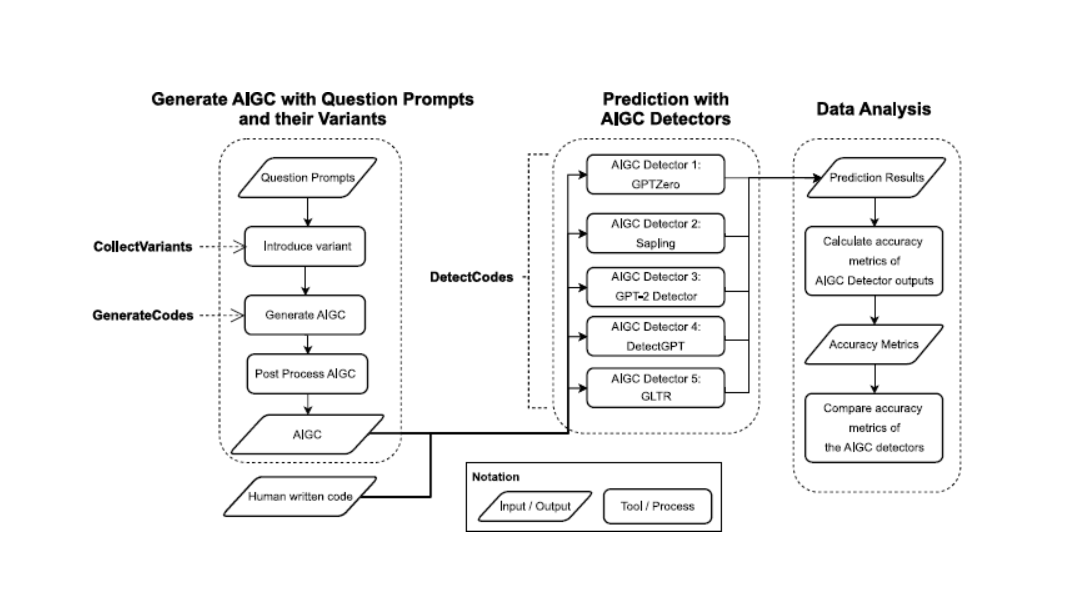
\includegraphics[width=1.00\linewidth]{fig1.png}
 %  \caption{Workflow of the AIGC and their variants’ generation process, AIGC prediction %with AIGC Detectors, and comparative
%analysis of AIGC Detector outputs with accuracy metrics.}
%\end{figure}
%\\

\section{Comparison with the Selected Paper}
\begin{table}[htbp]
\centering\small
\begin{tabular}{|p{2.4cm}|p{4.4cm}|p{5.4cm}|}\hline
\textbf{Approach} & \textbf{Focus} & \textbf{Relationship to NeRF-DA} \\\hline
Deblur-NeRF & Joint deblurring and radiance-field reconstruction. & Supplies the deblurring foundation; NeRF-DA adds selective training-data curation. \\\hline
DP-NeRF & Reconstruction from degraded images. & A baseline discussed in the supplied report; the original publication should be cited before final submission. \\\hline
ActiveNeRF & Active selection of views for reconstruction. & Related view-selection approach; the original publication should be cited before final submission. \\\hline
NeRF-DA & Active learning for radiance-field deblurring. & Selected paper: combines image selection, deblurring, and viewpoint augmentation.\cite{bib1} \\\hline
\end{tabular}
\caption{Qualitative comparison of related approaches.}
\end{table}
